
\Problem{Coloració de grafs}

\Statement

Donat un graf no dirigit, una coloració d'aquest graf és una assignació de
colors a cadascun dels vèrtexs del graf de forma que cap aresta tingui extrems
del mateix color. El nombre cromàtic d'un graf és el mínim nombre de colors
necesaris per colorar un graf donat.

\medskip

Com que trobar el nombre cromàtic d'un graf és computacionalment molt costós,
en aquest problema usarem un algorisme golafre que sol trobar una coloració
prou bona:

\medskip

Considerant que els vèrtexs i els colors venen identificats per nombres de
zero a $n-1$,  l'algorisme golafre agafa els vèrtexs seqüencialment (per ordre
d'identificador) i els coloreja amb el color més baix possible amb el qual no
s'hagi colorejat ja algun dels seus veïns.

\medskip

Per exemple, el nombre de colors emprats per l'algorisme golafre al graf
següent (el primer dels jocs de proves públics) és 4:

\begin{center}
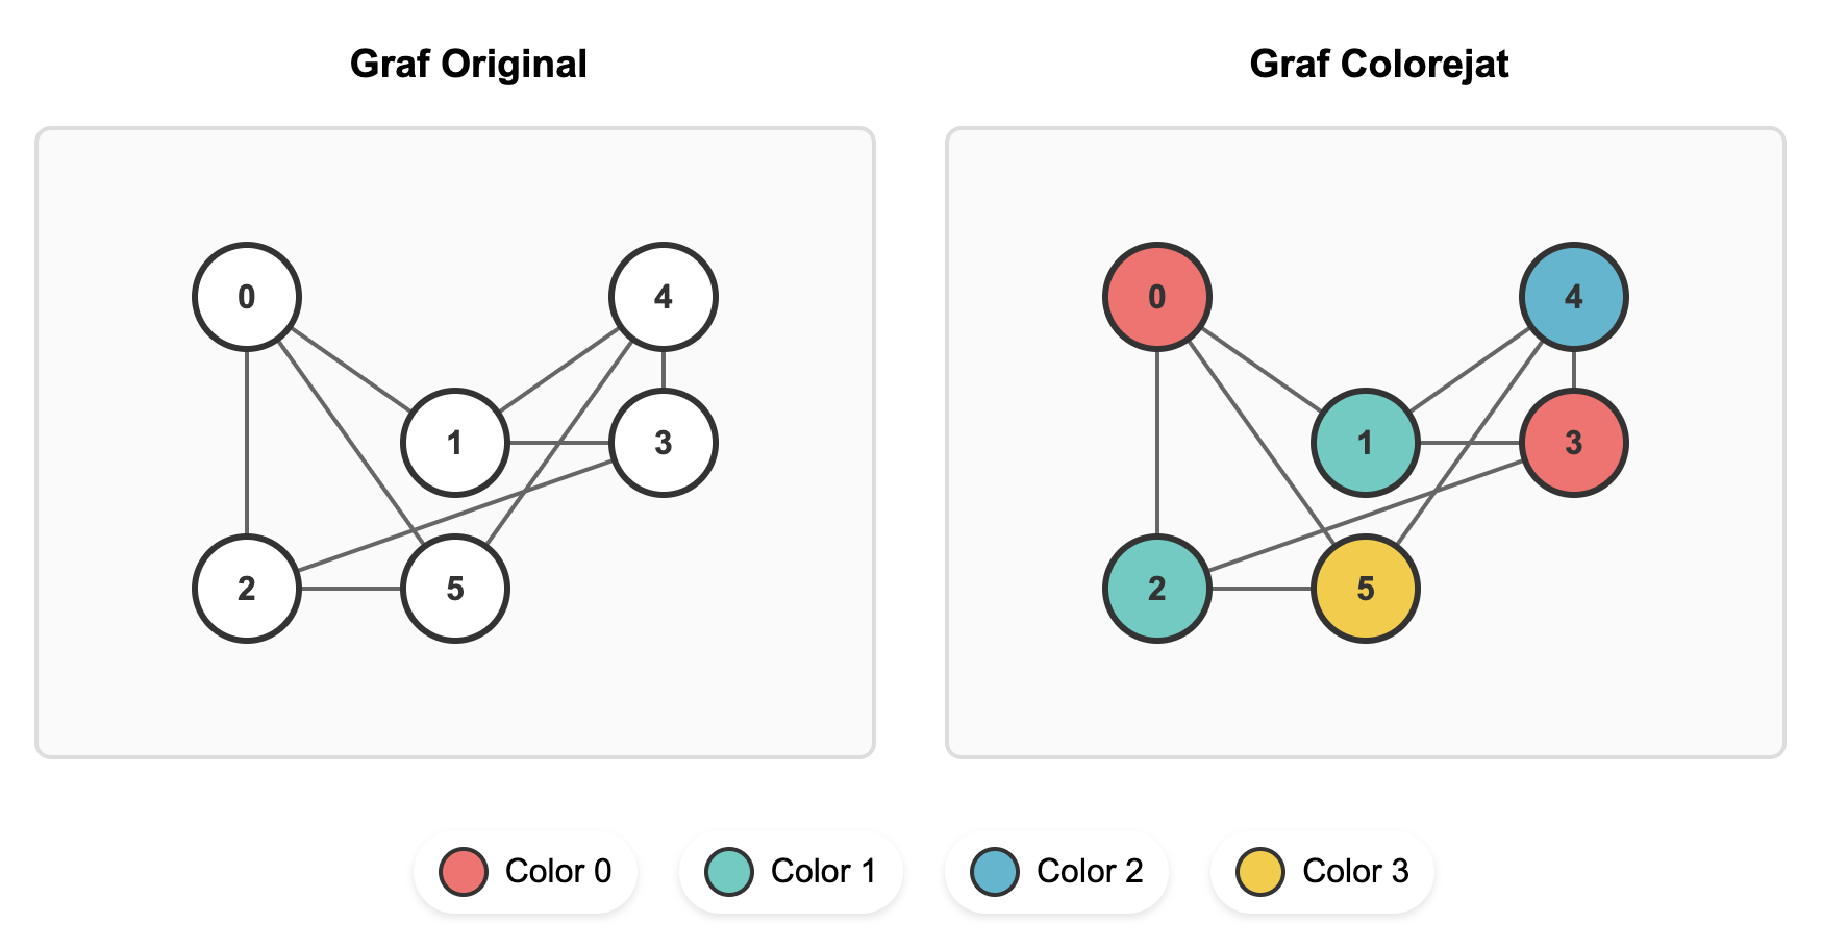
\includegraphics[width=0.75\textwidth]{exemple}
\end{center}


\Input

L'entrada conté diferents grafs (potser cap). Cadascun comença amb $n$ i $m$,
corresponent al nombre de vèrtexs i arestes del graf. Segueixen $m$ parells
$u,v$, indicant que hi ha una aresta entre $u$ i $v$. Es té que $n>0$, que
$0\le u < v <n$ i que no hi ha arestes repetides.
Suposeu que els grafs no són densos.

\Output

Per a cada graf, escriviu el nombre de colors emprats per l'algorisme golafre.


\Sample
